\documentclass{article}
\usepackage{graphicx}
\usepackage{xcolor}
\usepackage{listings}
\usepackage[ruled,vlined]{algorithm2e}
\usepackage{tikz}

\usepackage{xeCJK}
    \xeCJKsetup{AutoFakeBold=true, AutoFakeSlant=true}
    \setCJKmainfont{標楷體}
    \setmainfont{Times New Roman}

\definecolor{backgroundColour}{rgb}{0.95,0.95,0.92}
\definecolor{mGray}{rgb}{0.5,0.5,0.5}
\definecolor{mGreen}{rgb}{0.1,0.5,0.1}

\definecolor{mPurple}{rgb}{0.58,0,0.82}
\definecolor{backgroundColour}{rgb}{0.95,0.95,0.92}


\lstdefinestyle{CStyle}{
    backgroundcolor=\color{backgroundColour},   
    commentstyle=\color{mGreen},
    keywordstyle=\color{magenta},
    numberstyle=\tiny\color{mGray},
    stringstyle=\color{mPurple},
    basicstyle=\footnotesize,
    breakatwhitespace=false,         
    breaklines=true,                 
    captionpos=b,                    
    keepspaces=true,                 
    numbers=left,                    
    numbersep=5pt,                  
    showspaces=false,                
    showstringspaces=false,
    showtabs=false,                  
    tabsize=2,
    language=C
}

%%%% USERFUL FUNCTION
\newcommand{\alg}[1]{\textsc{\bfseries \footnotesize #1}}


\begin{document}

	\begin{titlepage}
		\centering
		\vspace*{1cm}
		\Huge
		\textbf{Data Structure}
		
		\vspace{0.5cm}
		\LARGE
		Homework2:連結串列交換首尾與反轉
		
		\vspace{2cm}
		\textbf{Author:} B11002220 CHI-CHUN, LO
		
		\vspace{1cm}



		\textbf{Date: }October 7, 2023
		
		\vfill
		
    	
\includegraphics[width=1\textwidth]{logo.png}
		
		\vspace{2cm}
		NTUST ECE
		
	\end{titlepage}
	\pagebreak
	% 目錄
	\tableofcontents
	
	
	% Problem page 
	\pagebreak
	\section{Problem}	
			Consider a linked list in which each node contains a word. Give a program that
		receives a word sequence and two integers. A and B, and constructs and prints the
		new list according to the following action:
		\begin{enumerate}
			\item Exchange the initial and final elements in the linked list.
			\item Reverse a sublist starting from A and ending at B.
		\end{enumerate}
	\subsection{Definition}
		首先,根據題目要求,我們可以定義以下單向連結串列結構且每個結構內都要能存放單詞:
		\begin{lstlisting}[style=Cstyle]
			typedef struct node *listPointer;
			typedef struct node
			{
				char *word;
				listPointer next;
			} node;
		\end{lstlisting}
      	接著,我們可以定義一個函數交換首尾的單詞Exchange,它的輸入是這個結構的頭,沒有輸出:
	     \begin{lstlisting}[style=Cstyle]
			void exchange(listPointer first)
		 \end{lstlisting}
		再來,討論如何反轉子串列。我們可以定義一個函數Reverse,它的輸入是這個結構的頭,有輸出1或0表示是否完成反轉:
		\begin{lstlisting}[style=Cstyle]
			int Reverse(listPointer *first)
		\end{lstlisting}
		 另外要特別注意由於反轉子串列的方式可能會涉及到串列的頭修改,因此這邊是用指標的方式去訪問。
	\subsection{Details}
		考慮各個函數的細節。
		\subsubsection{Exchange function}
			 由於實體的交換函數考慮的難度比較複雜,因此我們先討論交換節點的內容。exchange 函數它的輸入是串列的頭指標,因此我們需要做下面幾件事情完成這項功能:

			\begin{enumerate}
				\item 首先,考慮是否為空串列,如果是空串列,則直接返回。
				\item 再來,用一個指標指向最後一個節點
				\item 最後,交換首尾節點的內容
			\end{enumerate}
		\subsubsection{Reverse function}
			我們的Reverse函數的輸入是串列的頭指標。我們需要考慮多種情況,來滿足題目要求。
			下面是幾種可能會發生的情況;
		\begin{enumerate}
			\item 從0到length-1反轉,稱作完全反轉情況。

			\item 從0到length-i反轉,這邊稱作不完全反轉情況。Note: 1 < i < length 
			\item 從i到m反轉,這邊稱作通用情況。Note:這邊的0<i<m<length。
		\end{enumerate}
	
		針對從0到length-1反轉,我們可以透過討論反轉"I am a boy"的文字進行\texttt{reverse(\&first,0,3)}
		的情況來解決:

		\begin{enumerate}
			\item 先把第i+1的節點指向第i個節點直到第i+1的節點是end節點
			\item 再把first指向的節點end指向的節點(目的是為了把起頭改位置)
			\item 最後把start節點指向null後一個節點
		\end{enumerate}


		針對從0到length-i反轉,我們可以透過討論反轉"I am a boy"的文字進行\texttt{reverse(\&first,0,2)}
		的情況來解決:

		\begin{enumerate}
			\item 先把第i+1的節點指向第i個節點直到第i+1的節點是end節點
			\item 再把first指向的節點end指向的節點(目的是為了把起頭改位置)
			\item 最後把start節點指向end後一個節點
		\end{enumerate}

		最後,我們透過討論begin非0的反轉"I am a boy"的文字進行\texttt{reverse(\&first,1,3)}
		的情況來解決:
		\begin{enumerate}
			\item 先把第i+1的節點指向第i個節點直到第i+1的節點是end節點
			\item 再把start-1節點指向的節點end指向的節點
			\item 最後把start節點指向end後一個節點
		\end{enumerate}
		\pagebreak
		因此把這三個情況都做出來,我們就可以完成這道題目。針對不同情況的圖片請參考下面的圖:
		\begin{figure}[h]
			\centering
			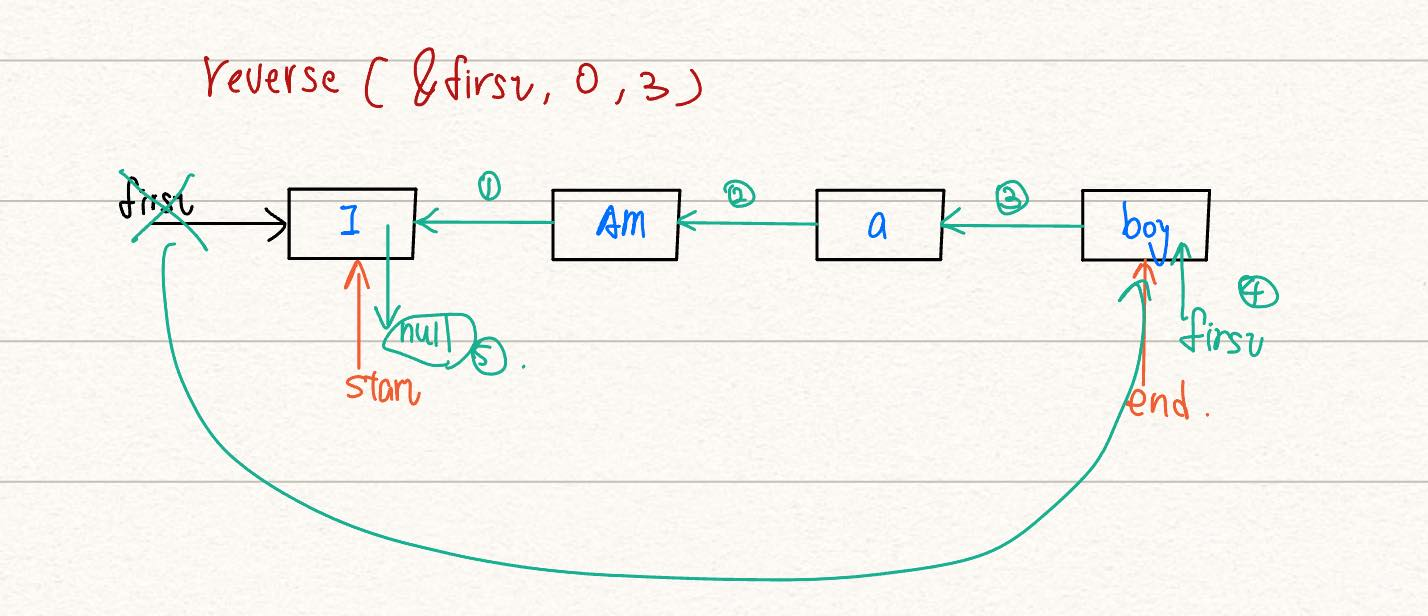
\includegraphics[height=4cm]{figure2.jpg}
			\caption{0 - length-1 reverse situation}
			\label{fig:example1}
		\end{figure}
		
		\begin{figure}[h]
			\centering
			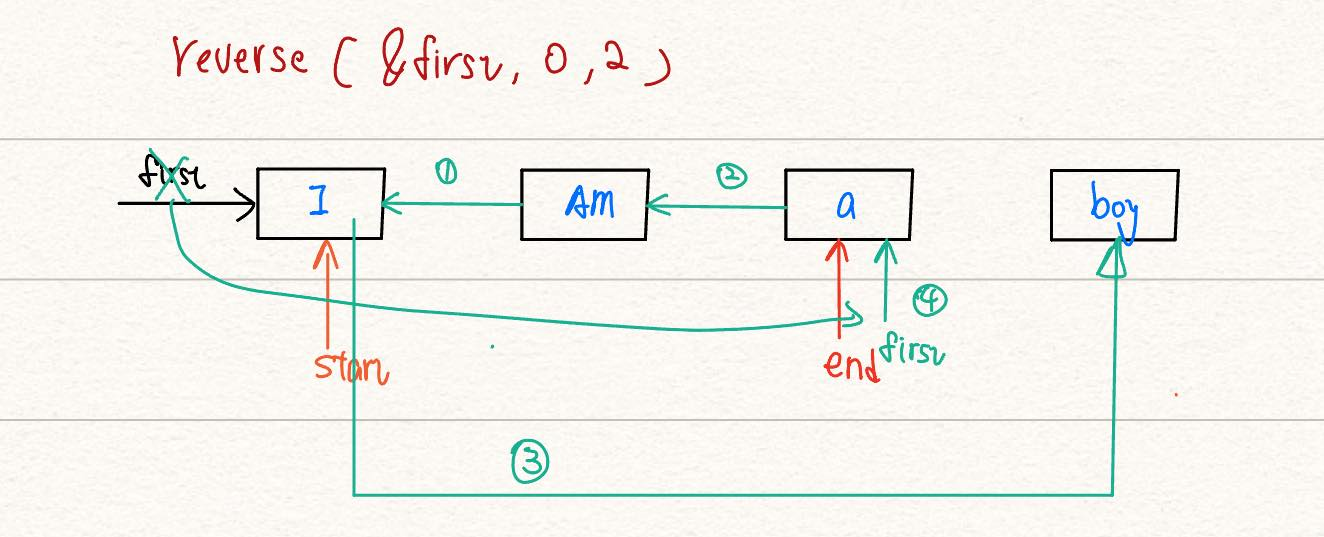
\includegraphics[height=4cm]{figure1.jpg}
			\caption{0 - length-i reverse situation}
			\label{fig:example2}
		\end{figure}
		
		\begin{figure}[h]
			\centering
			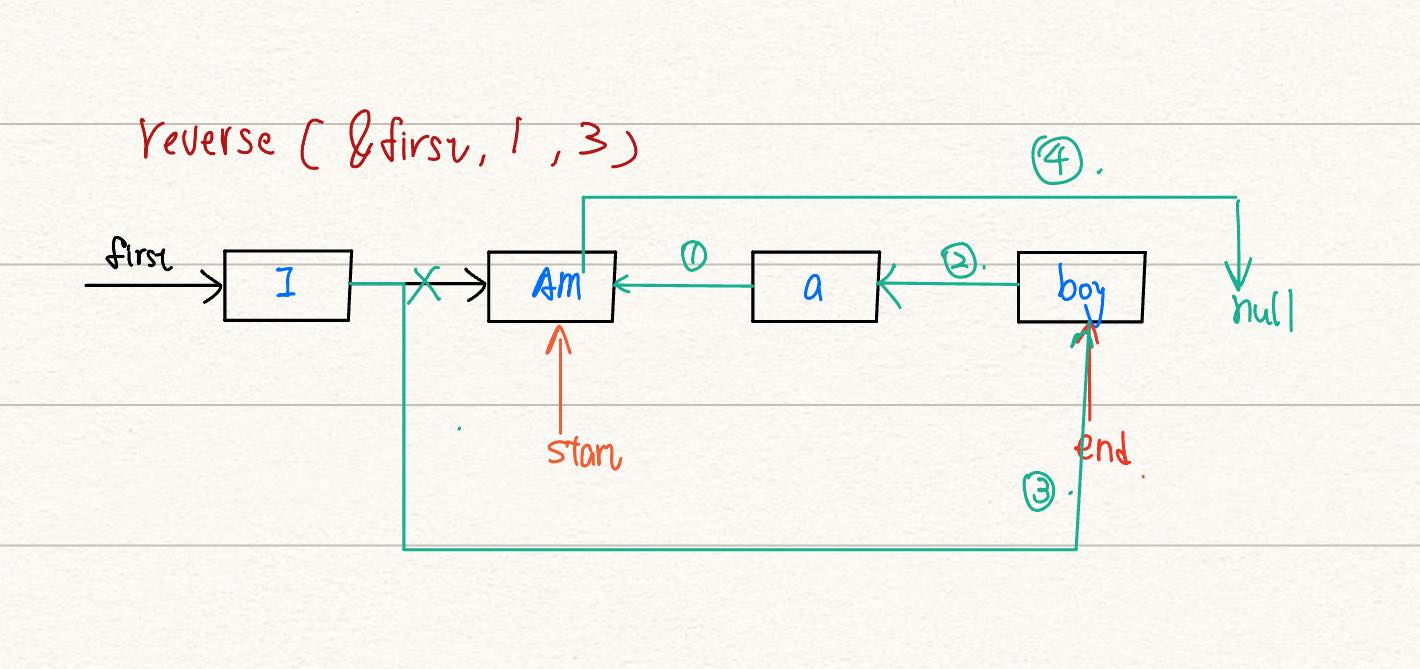
\includegraphics[height=4cm]{normal.jpg}
			\caption{n - m reverse situation}
			\label{fig:example3}
		\end{figure}
		

	\pagebreak
	% Code
	\section{Code}	
		下面是針對exchange()函數的程式碼。最主要的功能就是先判斷是否為空的list,再針對頭節點與尾節點的資料交換。如下:
		\begin{lstlisting}[style=CStyle]
			void exchange(listPointer first)
			{
				if (first == NULL || (first)->next == NULL)
				{
					return;
				}
				listPointer temp = first;
				for (; temp->next; temp = temp->next); // FIND THE LAST node 
				// exchage the first one with last
				char* Ctemp = _strdup((first)->word);
				(first)->word = _strdup((temp)->word);
				(temp)->word = Ctemp;
			}
		\end{lstlisting}
		第二部分是reverse()函數,主要功能是將list中的指定範圍的資料進行反轉。原則上功能大致分成四部分  
		,首先會先將錯誤的資料排除,接者針對要反轉的範圍反轉,最後設定start跟end指向的位置。如下:
		\begin{lstlisting}[style=CStyle]
			int reverse(listPointer* first, int begin, int end){
			int count = 0;
			listPointer node_before_start = NULL, node_after_end = NULL;
			listPointer start_node = NULL, end_node = NULL, temp = NULL;
			int length = get_length(	*first);
			// escape some error case
			if (begin > end || length <= end)
				return 0;
			else if (begin == end) /
				return 1;
			// set 4 point 
			for (temp = *first, count = 0; temp; temp = temp->next)
			{
				if (count == begin - 1)
					node_before_start = temp;
				if (count == begin)
					start_node = temp;
				if (count == end)
					end_node = temp;
				if (count == end + 1)
					node_after_end = temp;
				count++;
			}
			// start invert
			listPointer current, prev;
			current = start_node->next;
			prev = start_node;
			temp = NULL;
			// invert from start to end 
			while (current != node_after_end)
			{
				temp = current->next; // null
				current->next = prev; // student ->null
				prev = current;       //
				current = temp;
			}

			if (begin == 0 && length - 1 == end) // case 0 -length 
			{
				*first = end_node;
				start_node->next = NULL;
			}
			else if (begin == 0) // case 0-length-i
			{ // 0 - length - i
					*first = end_node;
					start_node->next = node_after_end;
			}
			else // case other 
			{
				node_before_start->next = end_node;
				start_node->next = node_after_end;
			}

			return 1;
            }
		\end{lstlisting}
	\section{Result}
	在這邊我們會針對不同的例子去測試程式的穩定性、正確性。
	\begin{itemize}
		\item \textbf{example1:} 討論在正常情況下的運作從頭開始
		
		\textbf{Input:}
		\begin{lstlisting}
			0 3
			Person real value first 
		\end{lstlisting}
		\textbf{Output:}
		\begin{lstlisting}
			first real value Person 
			Person value real first 					
		\end{lstlisting}
		解釋:測試反轉0-3的功能是否正常,第二列的輸出0-3確實是第一列0-3的反轉
		
		\item \textbf{example2:} 討論在正常情況下的運作從第一個開始反轉 \\
		\textbf{Input:}
		\begin{lstlisting}
			1 3
			Person real value first 			
		\end{lstlisting}
		\textbf{Output:}
		\begin{lstlisting}
			first real value Person 
			first Person value real 								
		\end{lstlisting}
		解釋:測試反轉1-3的功能是否正常,第二列的輸出0-3確實是第一列0-3的反轉
		
		\item \textbf{example3:} 超過範圍測試
		
		\textbf{Input:}
		\begin{lstlisting}
			1 100
			Person real value first 
		\end{lstlisting}
		\textbf{Output:}
		\begin{lstlisting}
			first real value Person 
			-1			
		\end{lstlisting}
		解釋:交換的功能不會影響,但是反轉的範圍超過我們就不動作!
		
		\item \textbf{example4:} 測試長度為1的句子反轉與交換是否都能輸出
		
		\textbf{Input:}
		\begin{lstlisting}
			0 0
			Person 
		\end{lstlisting}
		
		\textbf{Output:}
		\begin{lstlisting}
			Person 
			Person 				
		\end{lstlisting}
		解釋:輸入單詞很短,只要範圍正確,不影響輸出結果。
		
	\end{itemize}
	
	
	% Discussion and Conclusion
	\section{Discussion}
	根據上述結果,我們可以針對每個例子的輸入、輸出和解釋進行分析和討論。
	\
	\begin{itemize}
		\item \textbf{example1:} 針對開頭反轉
		\item \textbf{example2:} 針對非開頭反轉
		\item \textbf{example3:} 輸入超過範圍,則直接返回
		\item \textbf{example4:} 針對句子長度只有1反轉(不會返回)
	\end{itemize}
	所以根據以上結果能大致囊擴大部分輸入的例子,但是我們的程式碼仍有一些小地方需要改進。\ \ 
	當前取得文字的函數我們目前是利用\textbf{fgets( , length, )}其中它需要我們先設定input.txt單行最多讀入的長度,但是這就造成另個問題理論上我們的reverse可以反轉0~sizeof(int)-1的長度,但是因為單行讀入的上限導致輸入的文字只能不超過上限<
	因此更不可能達到我們設定的理想範圍。唯一的解決方法就是將fgets()替換成String.h中的getline,這個函數可以動態為輸入文字分配空間,繞過剛剛的文字上限導致的單詞上限。

	\section{Conclusion}
	最後,儘管這次的程式比上次難度略微增加,但是經過這次的練習後,我對linklist的認法有著更加深刻的理解。並明白資料結構是個必須搭配程式與畫圖的學科。可以先針對解決簡單的例子,在拓展到更複雜的例子查看是否可執行與遺漏。
\end{document}
